\documentclass[11pt,professionalfonts]{beamer}
\usefonttheme{serif}

\usepackage{presentation_packages}
\bibliography{library} % must be in the preamble when using biblatex package

\definecolor{mygray}{gray}{0.9}
\definecolor{RoyalBlue}{rgb}{0.25,0.41,0.88}
\def\Emph{\textcolor{RoyalBlue}}

\definecolor{tmp}{rgb}{0.804,0.941,1.0}
\setbeamercolor{numerical}{fg=black,bg=tmp}
\setbeamercolor{exact}{fg=black,bg=red}

\mode<presentation> 
{
  \usetheme{Warsaw}
  \usefonttheme{serif}
  \setbeamercovered{transparent}
}

\setbeamertemplate{footline}%{split theme}
{%
  \leavevmode%
  \hbox{\begin{beamercolorbox}[wd=.5\paperwidth,ht=2.5ex,dp=1.125ex,leftskip=.3cm,rightskip=.3cm plus1fill]{author in head/foot}%
    \usebeamerfont{author in head/foot}\insertshorttitle
  \end{beamercolorbox}%
  \begin{beamercolorbox}[wd=.5\paperwidth,ht=2.5ex,dp=1.125ex,leftskip=.3cm,rightskip=.3cm]{title in head/foot}
%    \usebeamerfont{title in head/foot}\mypaper\hfill \insertframenumber/\inserttotalframenumber
    \usebeamerfont{title in head/foot}\hfill \insertframenumber/\inserttotalframenumber
  \end{beamercolorbox}}%
  \vskip0pt%
} \setbeamercolor{box}{fg=black,bg=yellow}


\title[\texttt{ipython}]{\large \textbf{Ipython - Improved Python}}

\author{\vspace*{-0.3cm}}

   
\institute{
  \footnotesize
  {\normalsize\bf{Shankar Kulumani}}\\
  \vspace*{0.2cm}
    \textbf{Flight Dynamics \& Control Lab}\\ \vspace*{0.5cm}
  \begin{figure} %figure%
        
\includegraphics[width=0.75\textwidth]{figures/gw_txh_2cs_pos.pdf}
    \end{figure}
}
\date{}

\begin{document}
%=======================================================%

\setcounter{framenumber}{-1}
\begin{frame} %-----------------------------%
  \titlepage
\end{frame}   %-----------------------------%

\section*{}
\subsection*{Python Interpreter}  
\begin{frame}{Python Interactively}
    \begin{itemize}
        \item Python is an interpreted language - you can write and run code interactively
        \item Just try typing \texttt{python} at the Terminal
    \end{itemize}
    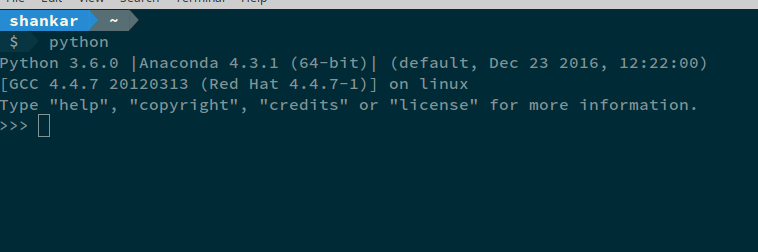
\includegraphics[width=\textwidth]{figures/python_interpreter.png}
\end{frame}

\begin{frame}{Python interpreter}
    \begin{itemize}
        \item Can write and run code directly here
        \item Doesn't offer some things that are very useful
            \begin{itemize}
                \item No autocompletion
                \item Debugging when there are errors
                \item Reading documentation or help from functions
            \end{itemize}
        \item There is a better way by using \texttt{ipython} - just another interpreter with some useful benefits
    \end{itemize}
\end{frame}

\begin{frame}{\texttt{ipython}}
    \begin{itemize}
    \item There is a lot of functionality - read the \href{http://ipython.readthedocs.io/en/stable/}{Documentation}
    \item Helpful Commands:
        \begin{itemize}
            \item Use tab for autocompletion - works by default
            \item \texttt{object?} - print details/help about an object
            \item \texttt{\%run script} - run your Python script
            \item \texttt{\%debug} - enter debugging after a crash
        \end{itemize}
    \item Using \texttt{ipython} and an editor gives you everything needed to write and run Python code
\end{itemize}
\end{frame}
\end{document}

